\section{Material und Methoden}

\subsection{Proband}
Alle hier dargestellten Daten beziehen sich auf eine männliche Person mit einer Körpergröße l~=~181 cm und einem Gewicht von m~=~75~kg. Neun Gelenke wurden mit Markern versehen, um diese später auszuwerten. Die Gelenke sind: Hals, Schulter, Ellenbogen, Handgelenk, Hüfte, Knie, Knöchel, Ferse und Ballen.

\subsection{Material}
HIER: TABELLE MIT KAMERA, SCHEINWERFERN, LAUFBAND, WAAGE ETC.\\
DANN NUR NOCH BILDER ZEIGEN FÜR DEN AUFBAU\\
AUSRICHTUNG DER KAMERA GENERELL ERKLÄREN
\subsubsection{Laufband}
Der Aufbau besteht aus einem mercury 4.0 Laufband (h/p/cosmos sports \& medical GmbH, Nussdorf-Traunstein, Germany), einer Samsung VP-HMX20C Videokamera (Samsung AG Seoul, Südkorea) und zwei weißen 500W Baustrahlern (MARKE???). Abbildung~\ref{fig:laufbnd_stp} (nicht maßstäblich) zeigt den Aufbau mit der Kamera XX~m vom Laufband entfernt. Die Bildebene ist parallel zur langen Kante des Laufbandes ausgerichtet.

\begin{figure}[h!]
	\centering
	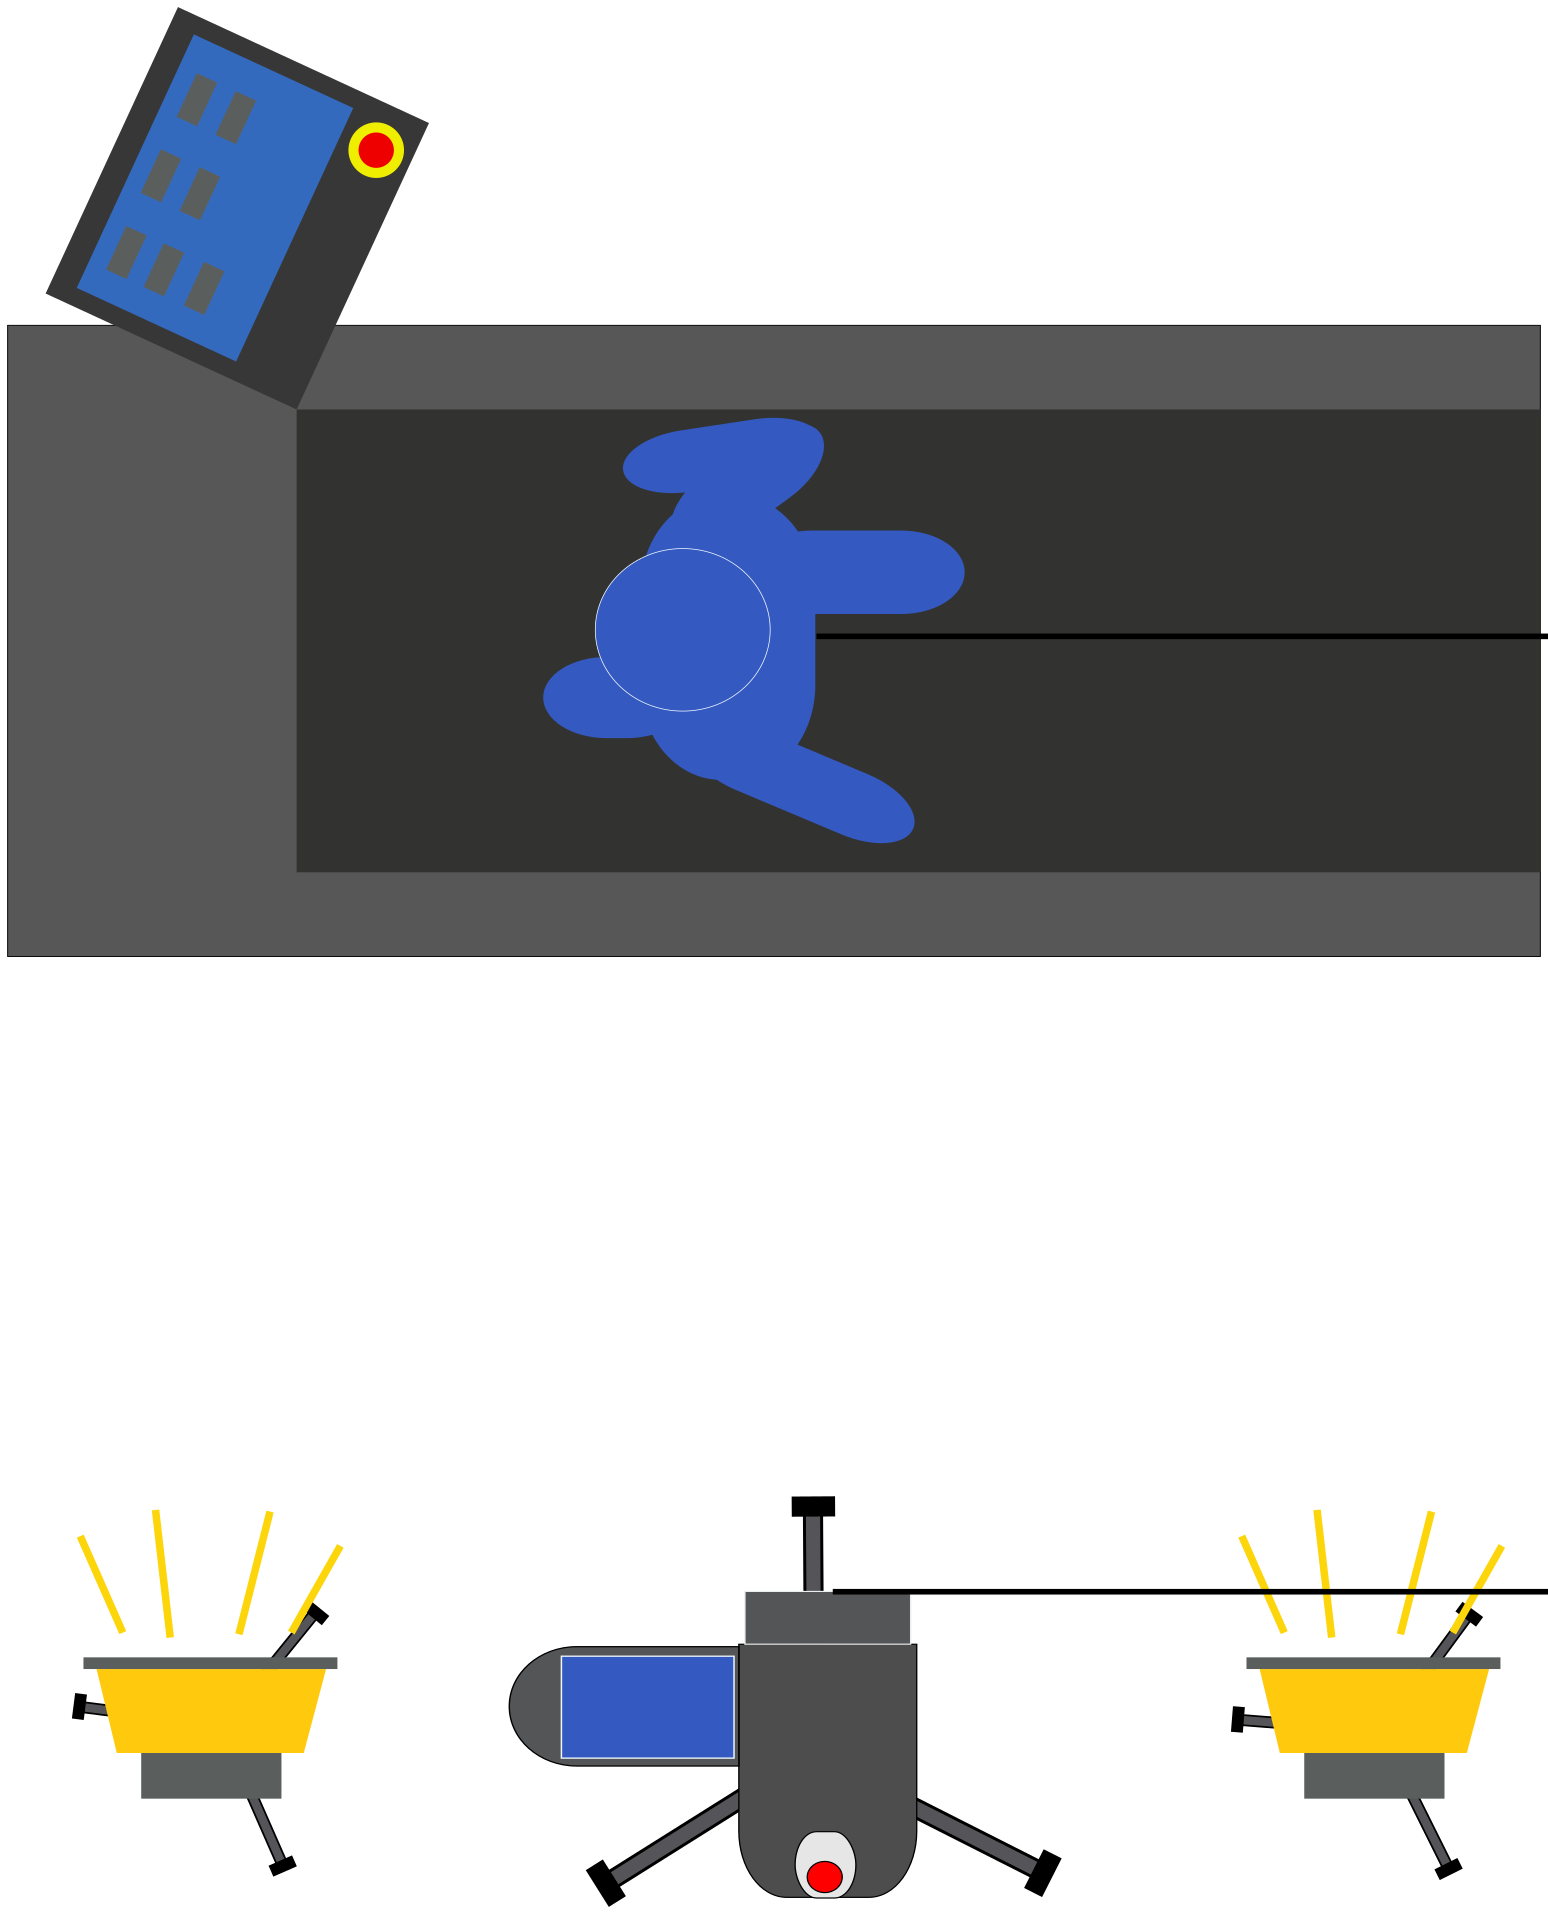
\includegraphics[width=0.5\linewidth]{bilder/mat_met/Laufband_setup}
	\caption[Aufbau Laufband Versuch]{Aufbau des Laufband-Versuches mit Laufband LB, Kamera K und Scheinwerfern SW Abstand zur Kamera $A_{Kam}~=~5~m$ }
	\label{fig:laufbnd_stp}
\end{figure}

\subsubsection{Laufsteg}
Dieselbe Videokamera und Baustrahler wie bei dem Laufband-Versuchen werden verwendet. Der Proband läuft in diesem Experiment über einen Laufsteg (Eigenbau Hochschule Bremen, Deutschland). In den Steg ist ein Quarzkristall-3-Komponenten-Dynanometer Typ 9257B (Kistler Gruppe Winterthur, Schweiz) zum Messen der Kräfte eingebaut, welches im Folgenden als Waage bezeichnet wird. Die Waage ist über einen Mehrkanal-Ladungsverstärker Typ 5070A (Kistler) mit einem Computer verbunden. Abbildung~\ref{fig:laufstg_stp} (nicht maßstäblich) zeigt den Aufbau mit der Kamera XX~m vom Laufsteg entfernt. Die Kamera steht zentriert vor der Waage und die Bildebene ist parallel zur langen Kante des Laufsteges ausgerichtet.

\begin{figure}[h!]
	\centering
	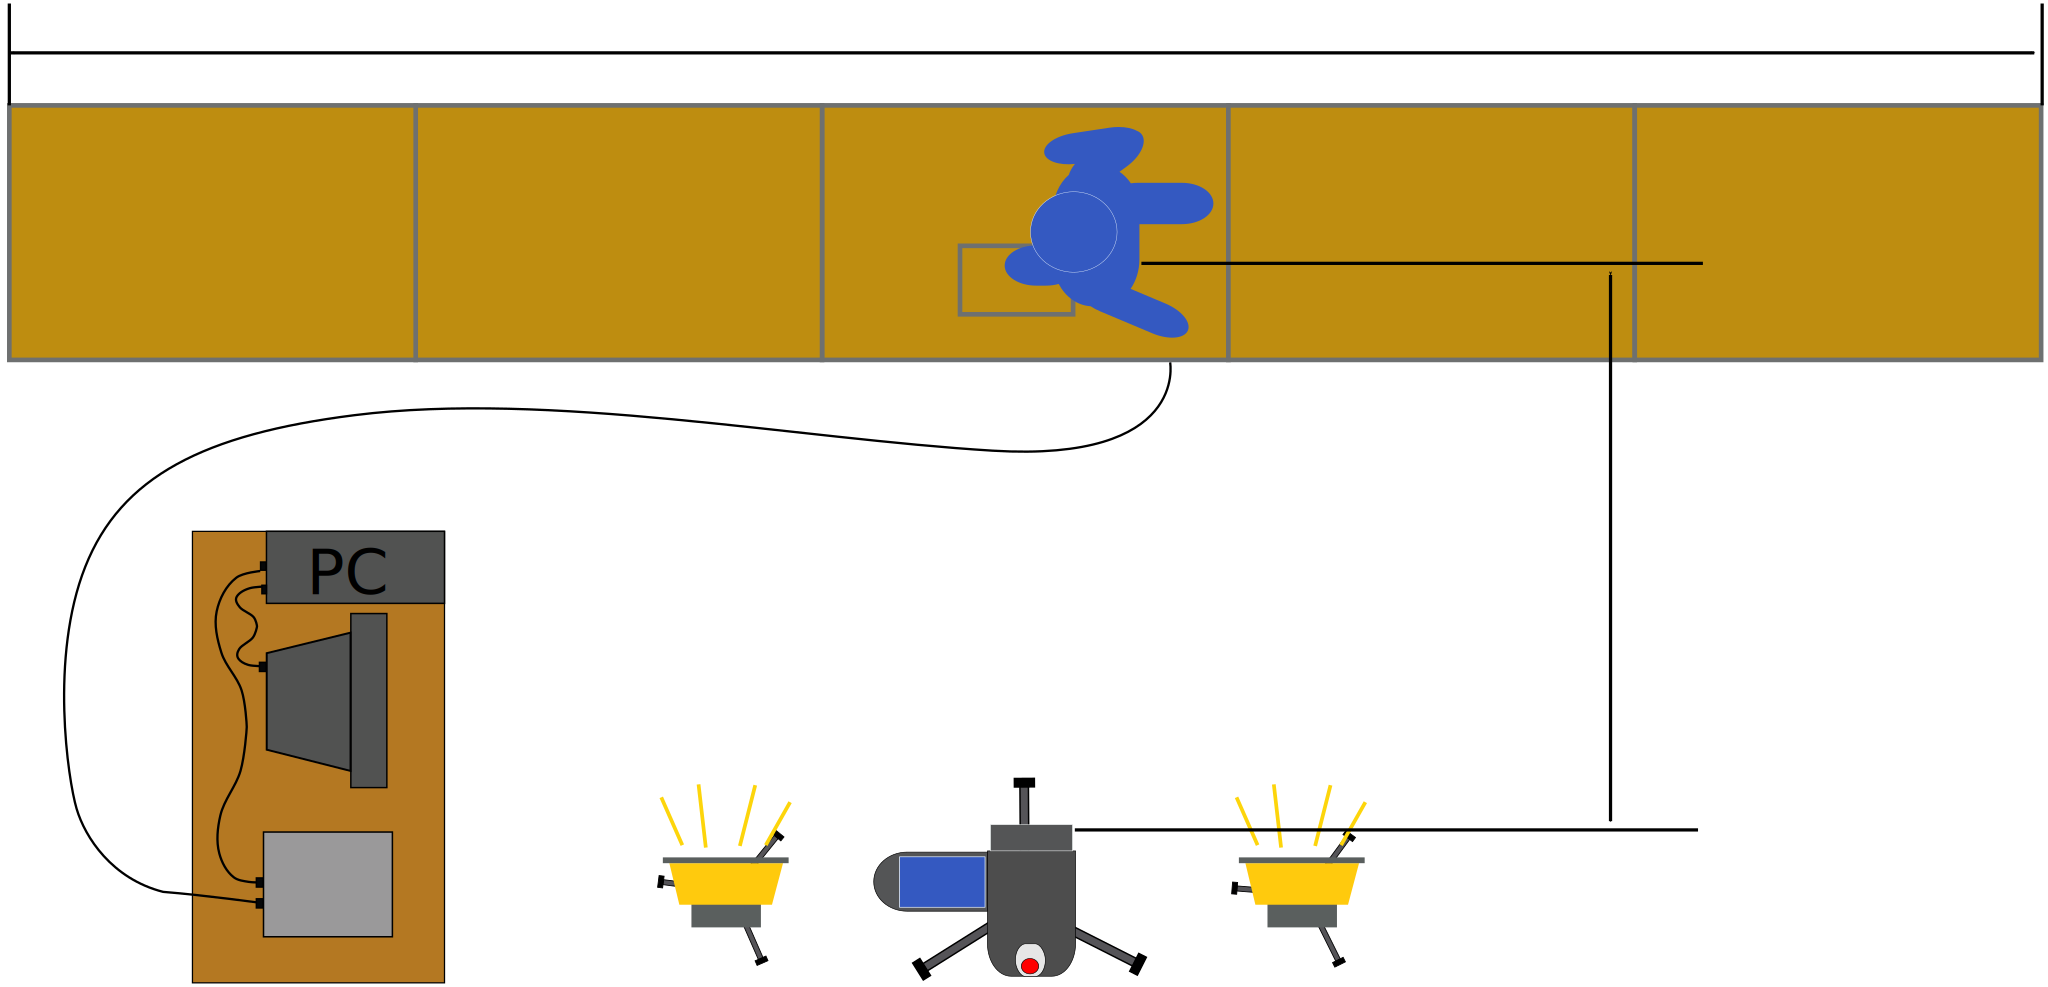
\includegraphics[width=0.7\linewidth]{bilder/mat_met/Laufsteg_setup}
	\caption[Aufbau Laufsteg Versuch]{Aufbau des Laufsteg-Versuches mit Laufsteg LS, Kamera K, Scheinwerfern SW, Computer C, Waage W und Ladungsverstärker LV. Länge Steg $L_S~=~6~m$ und Abstand zur Kamera $A_{Kam}~=~5~m$}
	\label{fig:laufstg_stp}
\end{figure}

\subsection{Methoden}
\subsubsection{Laufband}
Ausgehend von 1~km/h werden in 1~km/h-Schritten sieben Geschwindigkeiten untesucht. Das Gehen wird subjektiv von 1 (angenehm) bis 10 (unangenehm) bewertet.Je zwei Gangzyklen werden mit einer Bildrate von 50~Hz, einer Belichtung von 1/1000~s und auf 5~m fixierten Fokus aufgenommen.\\
Die Videos werden anschließend mit dem Programm ffmpeg 2.1 (LGP License, ffmpeg.org) in Einzelbilder zerlegt. In ImageJ (National Institutes of Health Bethesda, Maryland) werden mithilfe des Plugins MTrackJ \textbf{CITE(Meijering 20120)} die x- und y-Koordinaten aller Gelenke digitalisiert und im .mdf-Format gespeichert.

\subsubsection{Laufsteg}
EINSTELLUNGEN LADUNGSVERSTÄRKER???\\
Die Kameraeinstellungen vom Laufbandversuch übernommen finden auch hier Anwendung. Die Digitalisierung der Koordinaten ist wie oben beschrieben durchgeführt worden. Die Waagensignale werden mit 100 Hz und 200~N/V vom Ladungsverstärker an den Computer weitergeleitet. Mit DASYLab werden die Eingangssignale verarbeitet und alle 8 Kanäle im ASCII-Format gespeichert.
Für eine 4-Punkt-Kalibration wird die Waage in alle drei Raumrichtungen mit 0, 1, 3,6 und 7,75~kg belastet. Der Waagendrift wird über 60~s ohne Belastung für jede Raumrichtung ermittelt.\\
Blick geradeaus, um nicht auf den Gang nicht an die Waage anzupassen


\subsubsection{Datenauswertung mit Scilab}
Aufbau siehe Kirltey et al
Die Rohdaten der X- und Y-Koordinaten und der Waagenmessungen werden für beide Versuche in Scilab ausgewertet. Die verwendetete Vorgehensweise wird daher hier für beide Versuche gebündelt erklärt, um den Arbeitsvorgang deutlich darzustellen.\\\\
X/Y-Koordinaten\\
Glättung\\
Gleitender Mittelwer\\
Plotten\\
Berechnung Winkel\\
Berechnung Beschl.\\
Berechnung Geschw.\\
\\
Die acht Kanäle der Waage werden in X-, Y- und Z-Richtung zusammengefasst. Der Waagendrift wird durch lineare Regression ermittelt und von allen Rohdaten abgezogen.
Für die Kalibration werden die Signale für die vier Gewichte über 1000 Werte gemittelt. Dadurch können den Spannungen tatsächliche Gewichte zugeordnet werden, welche mittels linearer Regression eine Extrapolation für folgende Messungen erlauben. Die 
Waagendaten\\
Kalibration\\
offset in jeder Messung\\
Volt somit in N umgerechnet\\

Inverse Kinematik\\
FELIX WAS HAST DU DA ALLES GEZAUBERT?!?!?


alle rohdaten an scilab gegeben für beide Versuch eund dann asugewertet\\
Gleichungen angeben\\
Daten filtern!\\
\textit{Gleichungen angeben}\\
\textbf{Kalibrierung}\\
- Nullmessung zur Bestimmung des Waagendrifts\\
- Kalibrierungsmessung\\
--> Bestimmung der der Abhängigkeit zwischen Belastungskraft und Messdaten\\
- Reduktion des Waagendrifts\\
- Regressionsgleichung von Messdaten und Belastungskraft bestimmen\\
\textbf{Datenaufnahme}\\
- Kräfte zusammenfassen\\
- Waagendrift aus Rohdaten rausrechnen\\
- Mittels der Kalibrierungsgleichungen die Rohdaten in Kräfte umrechnen\\
\textbf{Skalierung und Synchronisation!!}\\
- Bei der Skalierung wird die Datenrate der Videorate angepasst (hier also nur jeder zweite Datensatz). Gegebenenfalls muss zwischen den Datensätzen interpoliert werden.\\
- Bei der Datensynchronisation findet ein Abgleich des Videomaterials und der Bodenreaktionskräfte statt\\
\textbf{Digitalisierung des Videomaterials}\\
- Skalieren der Videoaufnahme (ACHTUNG! Referenzbild mit Maßstab erforderlich?!?!?)\\
- Tracken von allen Gelenken\\
- Segmentschwerpunkte berechnen (Fuß, Unter- und Oberschenkel)\\
\textbf{Datenberechnung\ KINEMATIK??}\\
- Berechnung von linearen Geschwindigkeiten und Beschleunigungen\\
- Berechnung von Winkelgeschwindigkeiten und Winkelbeschleunigungen\\
\textbf{Datenfilterung (gleitender Mittelwert)}\\
- ACHTUNG! Je nach Anzahl von Stützstellen und Iterationen müssen Bilder vor und nach dem Schrittzyklus in die Digitalisierung einbezogen werden. z.B. 3 Stützstellen und eine Iteration benötigt 1 Bild vorher und ein Bild nachher, um i-1 und n+1 zu berücksichtigen.\\
\textbf{Kinetische Berechnungen (Wagenzentrum rausrechnen?)}\\
Auf der Grundlage von David A. Winter werden:\\
- Kräfte und Momente in den Gelenken berechnet\\
- Berechnung mittels inverser Dynamik\\